%Especificacion
\documentclass[12pt]{article}

%Paquetes
\usepackage[left=2cm,right=2cm,top=3cm,bottom=3cm,letterpaper]{geometry}
\usepackage{lmodern}
\usepackage[T1]{fontenc}
\usepackage[utf8]{inputenc}
\usepackage[spanish,activeacute]{babel}
\usepackage{mathtools}
\usepackage{amssymb}
\usepackage{enumerate}
\usepackage{graphicx}
\usepackage{titlesec}
\usepackage{enumitem}
\usepackage{alltt}
\usepackage{hyperref}
\usepackage[export]{adjustbox}

%Preambulo
\title{Seminario de Heurísticas de Optimización Combinatoria \\ Recocido Simulado con Aceptación por Umbrales}
\author{Andrea Itzel González Vargas}
\date{Facultad de Ciencias UNAM}

\setlength\parindent{0pt}

\begin{document}
\maketitle
En este proyecto se implementó la heurística del recocido simulado con aceptación por umbrales para la resolución del problema del agente viajero. Se cuenta con una base de datos en donde se guardan las ciudades a tomar en cuenta junto con sus respectivas conexiones con otras ciudades. \\
Para implementar el proyecto se utilizó en lenguaje de programación Go junto con el manejador de bases de datos SQLite3. \\
El repositorio del proyecto está en \url{https://github.com/andreagonz/recocido}
\subsection{Ejecución del programa}
Para poder ejecutar el programa se adjunta la imagen de máquina virtual de QEMU \textsf{manjaro.img}. Lo único que se tiene que hacer es correr la máquina con
\begin{verbatim}
    qemu-system-x86_64 -hda manjaro.img -m <memoria en bytes>
\end{verbatim}
Si de algo sirve, la contraseña de root es ``chepe''.
Una vez que se haya abierto la máquina, se deberá de ir al directorio \textsf{$\sim$/go/src/github.com/andreagonz/recocido}, donde se debe de correr \textsf{go build}, lo cual creará el archivo ejecutable \textsf{recocido}. \\
El comando para correr el programa es el siguiente:
\begin{verbatim}
    ./recocido <archivo.tsp> <params.txt> [ops]
\end{verbatim}
donde \textsf{<archivo.tsp>} es el archivo con el conjunto de ciudades cuya ruta mínima quiere encontrarse. El formato de éste archivo es escribir los índices de las ciudades como están en la base de datos separados por una coma y un espacio. Por ejemplo:
\begin{verbatim}
26, 37, 14, 7, 1, 27, 31, 2, 33
\end{verbatim}
\textsf{<params.txt>} es el archivo donde se especifica que parámetros se usarán para la ejecución. El formato del archivo es el siguiente:
\begin{alltt}
\{int: Semilla\}
\{int: Tamaño del lote\}
\{double: P\}
\{double: \(\epsilon\sb{p}\)\}
\{double: \(\epsilon\sb{t}\)\}
\{double: \(\epsilon\)\}
\{double: \(\phi\)\}
\{int: c\}
\end{alltt}
donde \textsf{\{t: X\}} es la representación numérica de \textsf{X}, es decir de cada parámetro, si \textsf{t} es \textsf{int} sólo se aceptarán números enteros, si es \textsf{double} se permite también decimales. Ejemplo:
\begin{verbatim}
30
500
0.9
0.001
0.0001
0.001
0.9
5
\end{verbatim}
Por último, \textsf{[ops]} son los parámetros opcionales del programa, hay dos de estos: \\

\textsf{-g}: Permite que se creé la gráfica de soluciones aceptadas. Se hará un archivo \textsf{costos.txt} y un archivo \textsf{costos.png}. \\

\textsf{-m}: Crea la representación en mapa de la ruta en el archivo \textsf{mapa.html}, donde se utiliza Google Maps. \\

Ejemplo de ejecución: 
\begin{verbatim}
    ./recocido archivos/prueba.tsp archivos/params/1.txt -m -g
\end{verbatim}

Al final de su ejecución, el programa crea un archivo llamado \textsf{ruta.tsp} donde se imprime la ruta de la mejor solución encontrada. \\

Si se quiere ver la documentación del proyecto, basta con ejecutar
\begin{verbatim}
    godoc -http=:6060
\end{verbatim}
y acceder desde el navegador a \textsf{localhost:6060/pkg/github.com/andreagonz/recocido/}

\newpage

\subsection{Diseño}
Se dividió el diseño en la parte genérica del recocido y la parte de implementación específica para el problema del agente viajero, de manera que se pueda reutilizar el código para algún otro problema. La parte genérica está implementada en \textsf{heuristica/heuristica.go}, donde se hace uso de las interfaces de Go para representar las soluciones de un lote y se implementaron los algoritmos del recocido para calcular el lote, la temperatura y la aceptación por umbrales. La parte orientada al problema del agente viajero está en \textsf{implementacion/solucion.go}, donde se implementaron los métodos de la interfaz \textsf{Solucion}. \\

Por otro lado se tiene otras funciones en \textsf{util/} que permiten manipular archivos, crear las gráficas y hacer los mapas.

\subsection{Experimentación}
Se toma en cuenta al directorio \textsf{$\sim$/go/src/github.com/andreagonz/recocido} como directorio base. \\
Para probar el programa fue proporcionado un conjunto de ciudades que están guardadas en \textsf{archivos/prueba.tsp}. \\

Se utilizaron 4 conjuntos de parámetros y se corrieron 50 semillas (de la 0 a la 49) distintas para cada uno.

\begin{center}
  \begin{tabular}{ |c||c|c|c|c|c| } 
    \hline
    Parámetro & Params1 & Params2 & Params3 & Params4 \\ [0.5ex] 
    \hline\hline
    $Lote$ & 500 & 500 & 500 & 1000  \\\hline 
    $P$ & 0.9 & 0.9 & 0.9 & 0.9 \\ \hline 
    $\epsilon_p$ & 0.01 & 0.001 & 0.001 & 0.001 \\ \hline 
    $\epsilon_t$ & 0.01 & 0.01 & 0.001 & 0.001 \\ \hline 
    $\epsilon$ & 0.01 & 0.001 & 0.001 & 0.001 \\ \hline 
    $\phi$ & 0.9 & 0.9 & 0.9 & 0.9 \\ \hline 
    $c$ & 5 & 5 & 5 & 5 \\ 
    \hline
  \end{tabular}
\end{center}

A continuación se mostrará los resultados que se obtuvo con cada conjunto de parámetros.

\newpage

\subsubsection*{Params1}
Con este conjunto de parámetros se obtuvo un $\%$36 de soluciones factibles. Se muestra la gráfica de número de semilla contra costo de la mejor solución obtenida con esa semilla. Tambien se puede ver si la solución es factible o no. \\

\begin{center}
  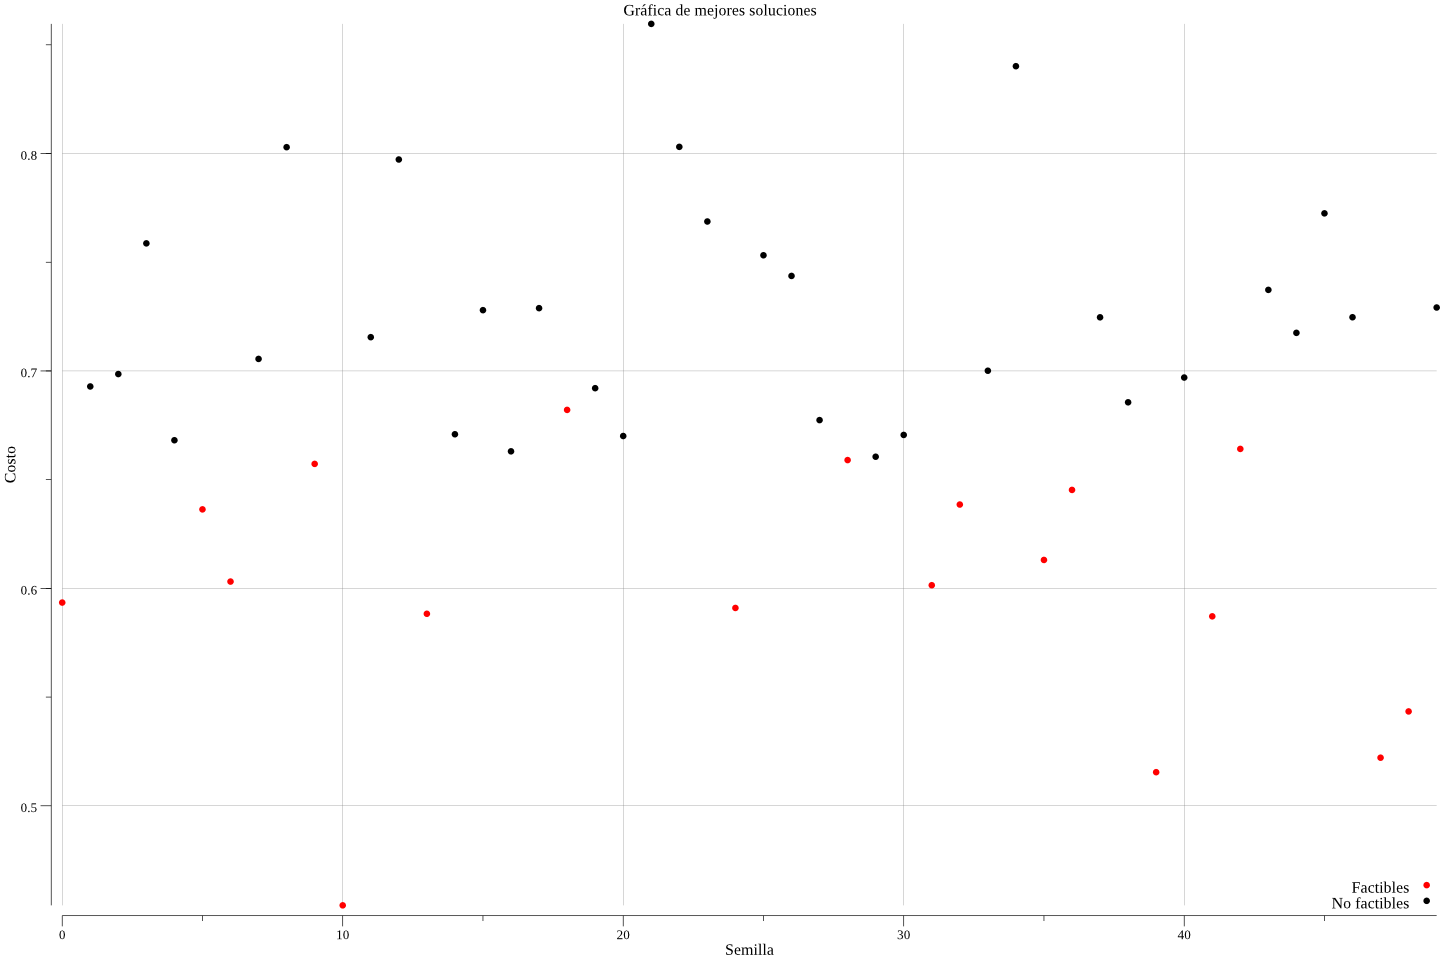
\includegraphics[scale=0.25]{../archivos/graficas/mejores-soluciones/soluciones1.png} \\
\end{center}
  
La mejor solución encontrada tuvo un costo de \textbf{0.454207349}, lo cuál es decente pero más alto de lo que nos gustaría y como se puede apreciar, es una ruta algo alejada de la óptima. Se obtuvo con la semilla \textbf{10}. \\

\begin{center}
  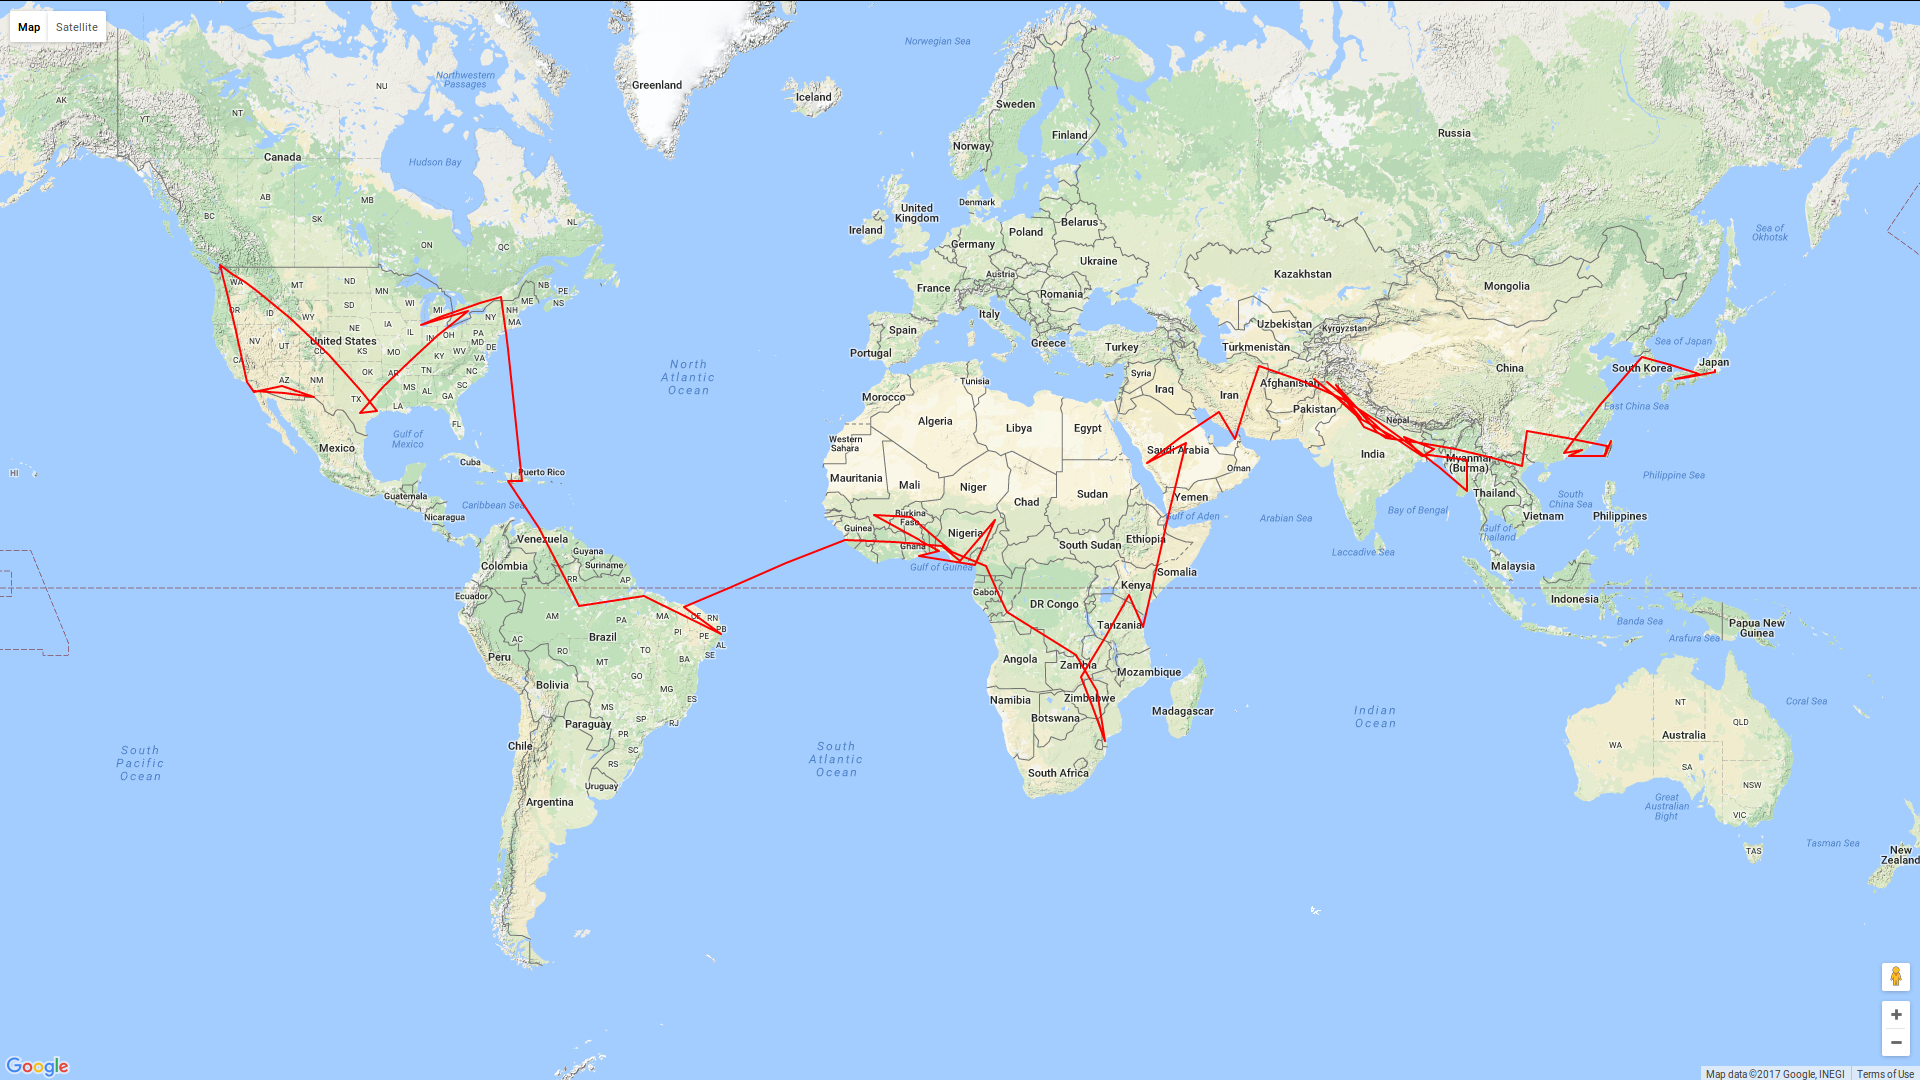
\includegraphics[scale=0.2]{../archivos/mapas/mapa1.png} \\
\end{center}

La gráfica del costo de las soluciones aceptadas de la mejor solución es la siguiente (se omitieron varias soluciones ya que eran demasiadas): \\

\begin{center}
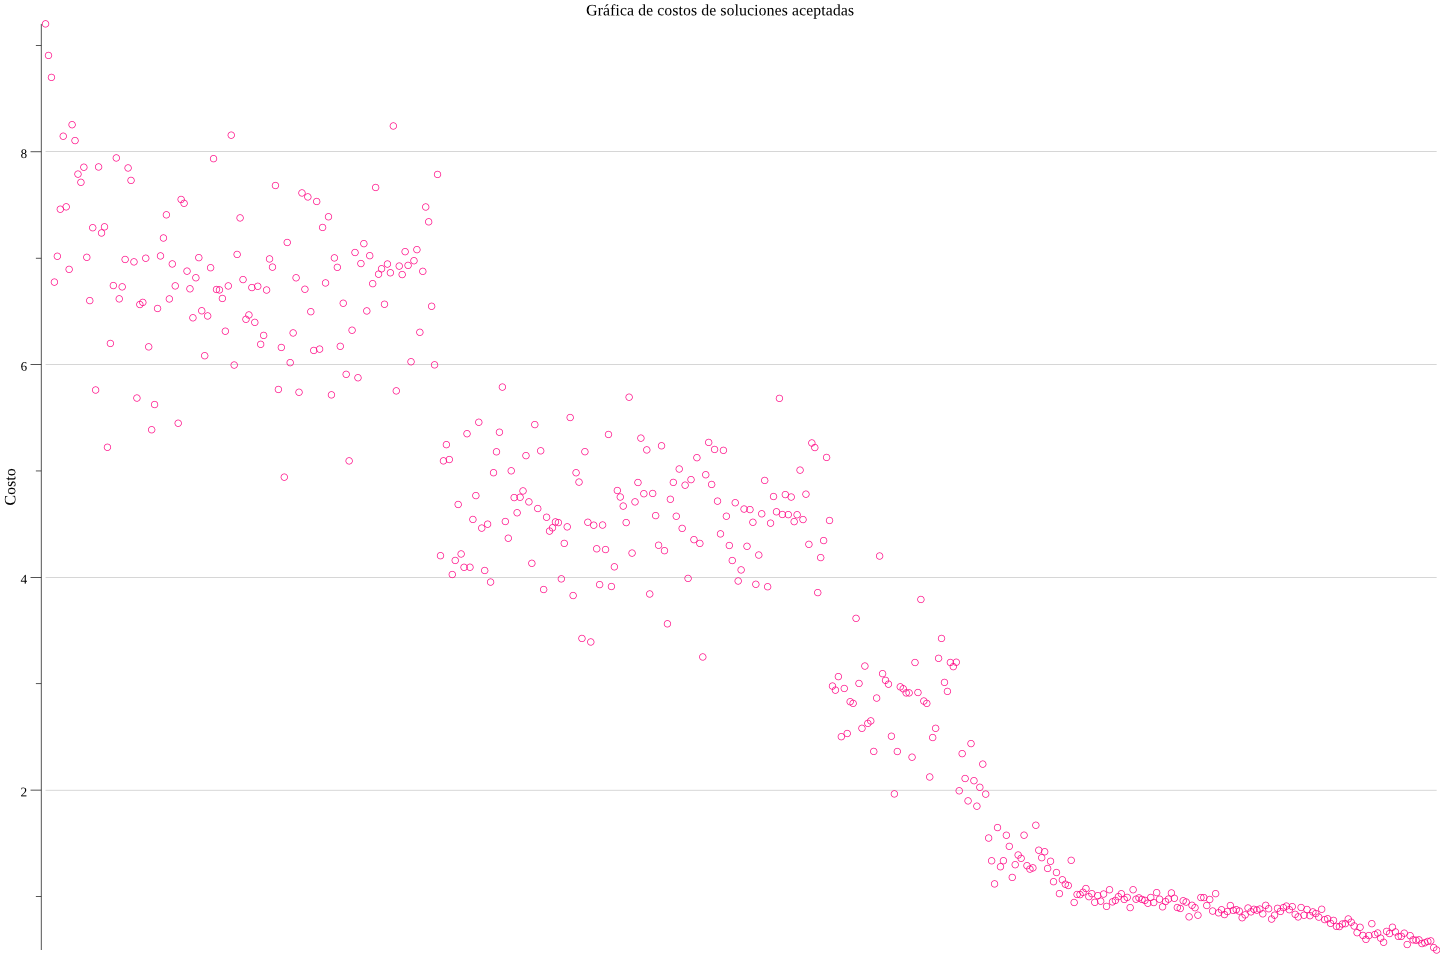
\includegraphics[scale=0.3]{../archivos/graficas/soluciones-aceptadas/costos1.png} \\
\end{center}

El promedio de los costos de las mejores soluciones de todas las semillas fue 0.681062436 \\

La mejor solución encontrada con Params1 se puede obtener con los parámetros \textsf{archivos/params/1.txt}.

\newpage

\subsubsection*{Params2}

Se obtuvo un $\%$66 de soluciones factibles, muchas más que en el caso anterior. \\
Las gráficas obtenidas son las siguientes: 

\begin{center}
  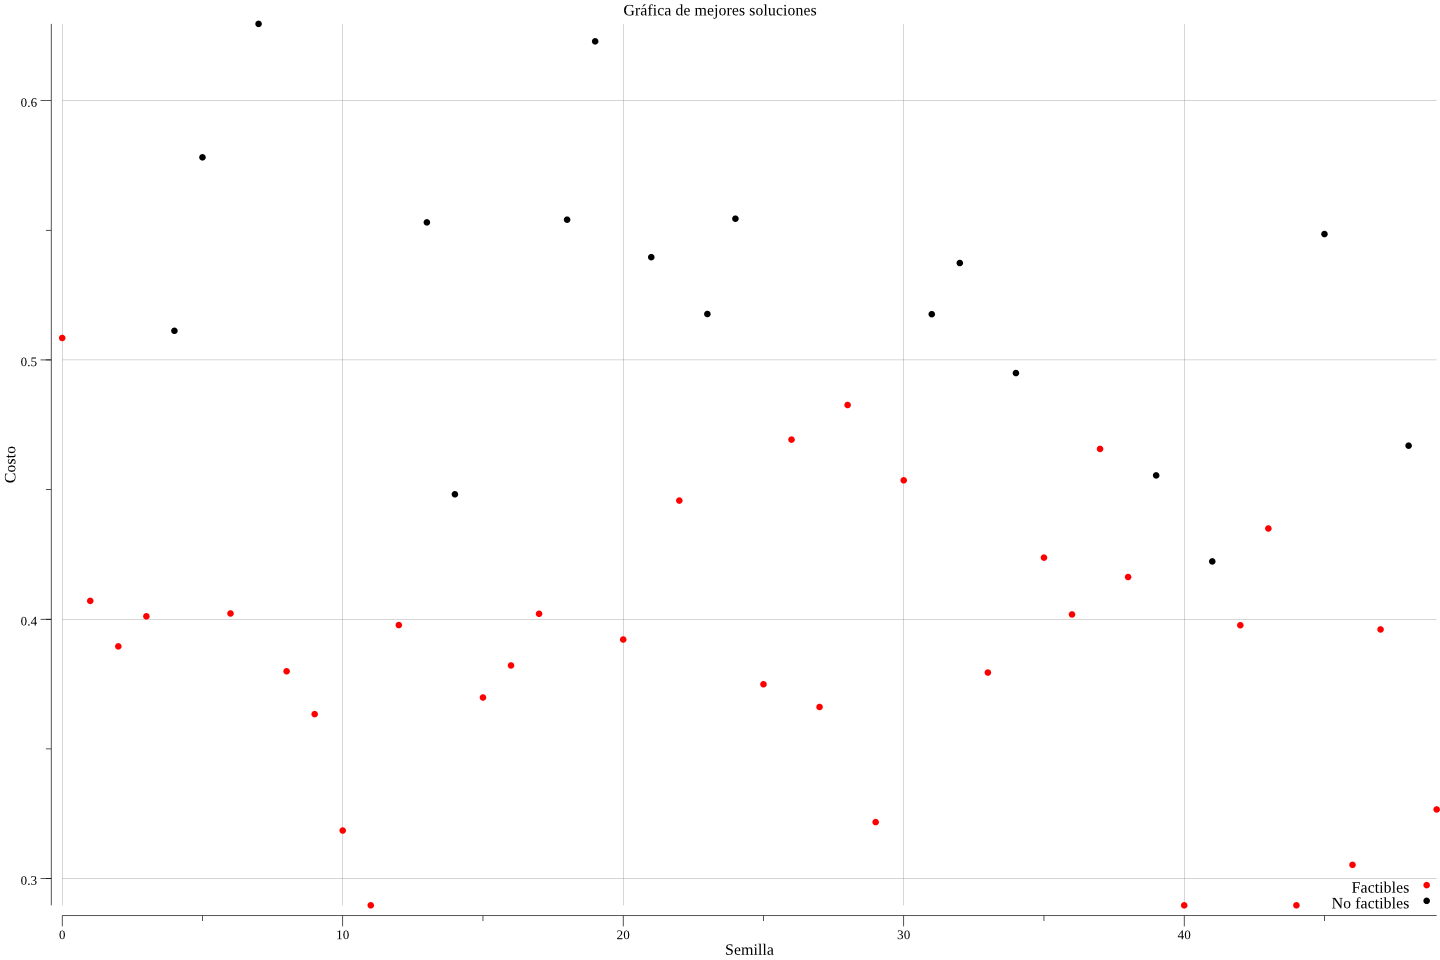
\includegraphics[scale=0.25]{../archivos/graficas/mejores-soluciones/soluciones2.png} \\
\end{center}
  
La mejor solución encontrada tuvo un costo de \textbf{0.289669266}, se obtuvo con la semilla \textbf{40}. Por lo que podemos ver en el mapa ésta pareciera ser la ruta óptima, sin embargo como veremos adelante se encontró una mejor.  \\

\begin{center}
  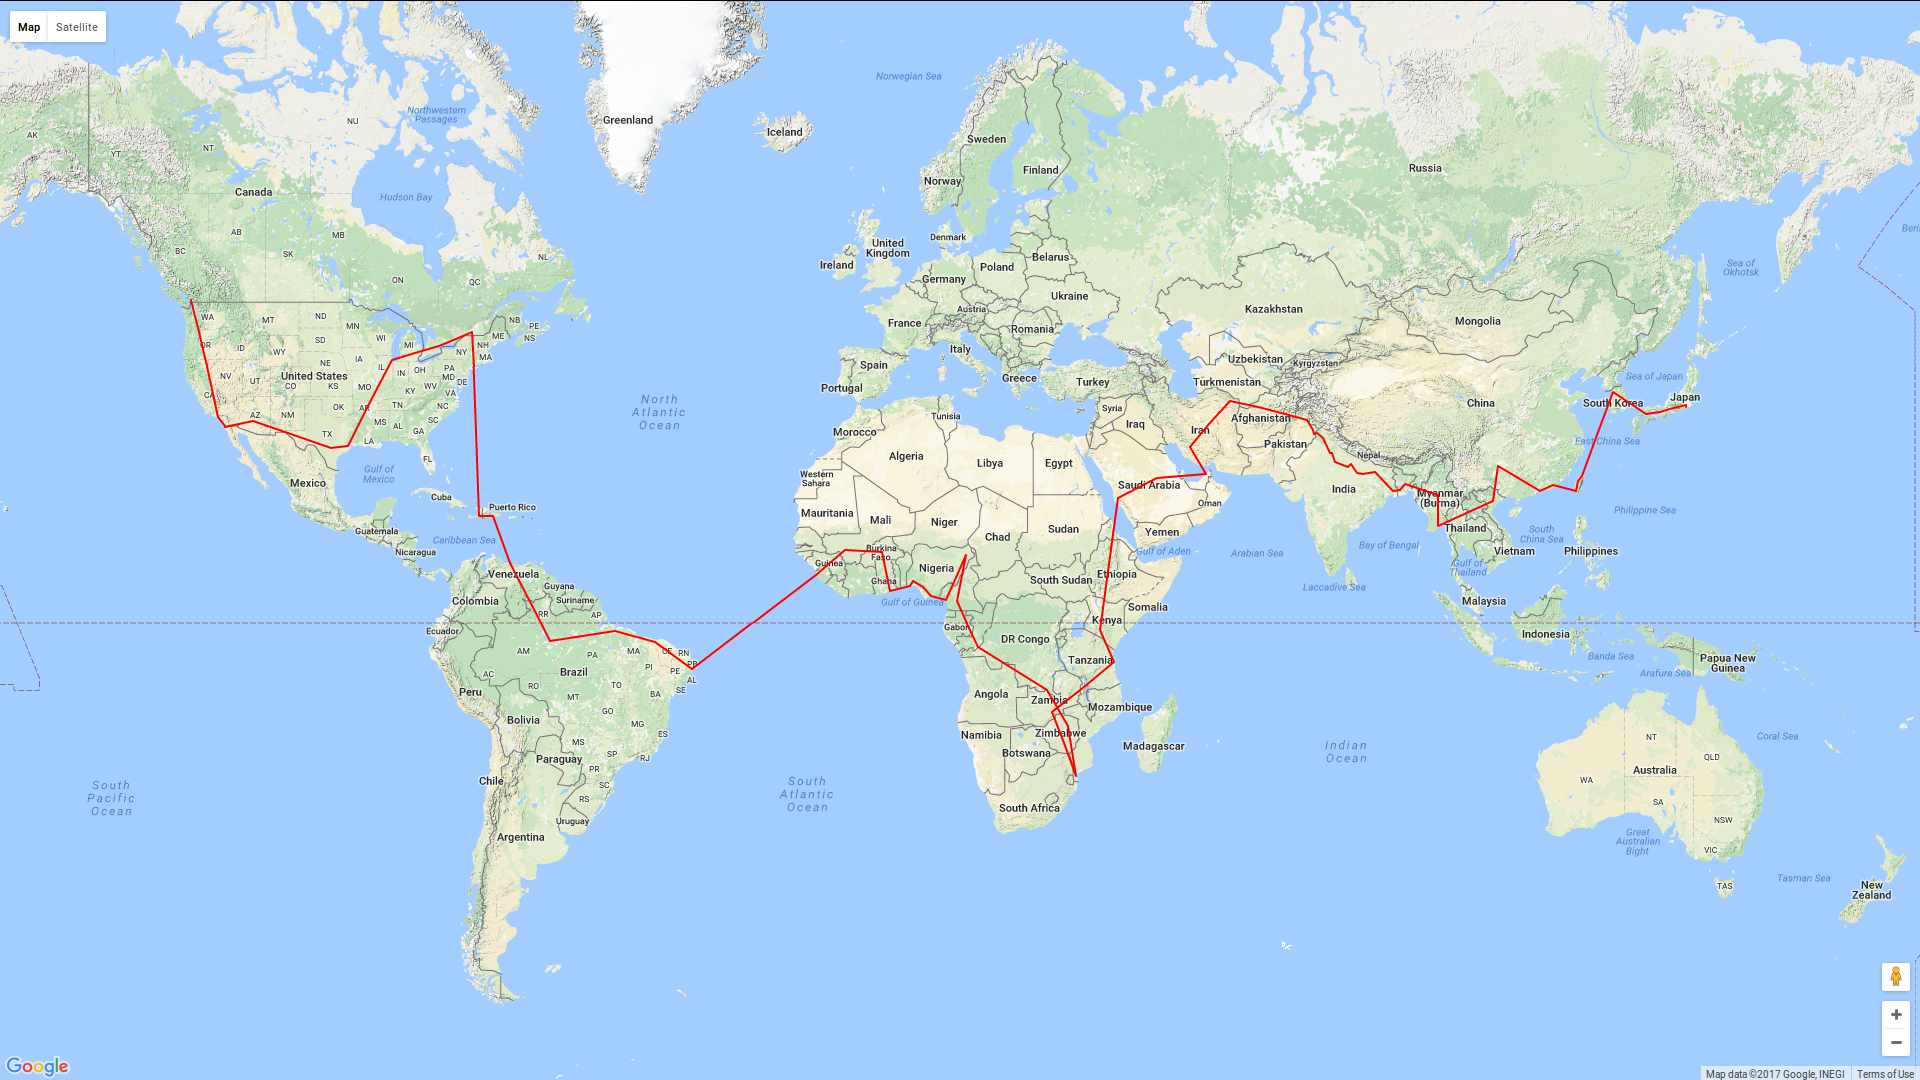
\includegraphics[scale=0.2]{../archivos/mapas/mapa2.png} \\
\end{center}

Gráfica del costo de las soluciones aceptadas de la mejor solución: \\

\begin{center}
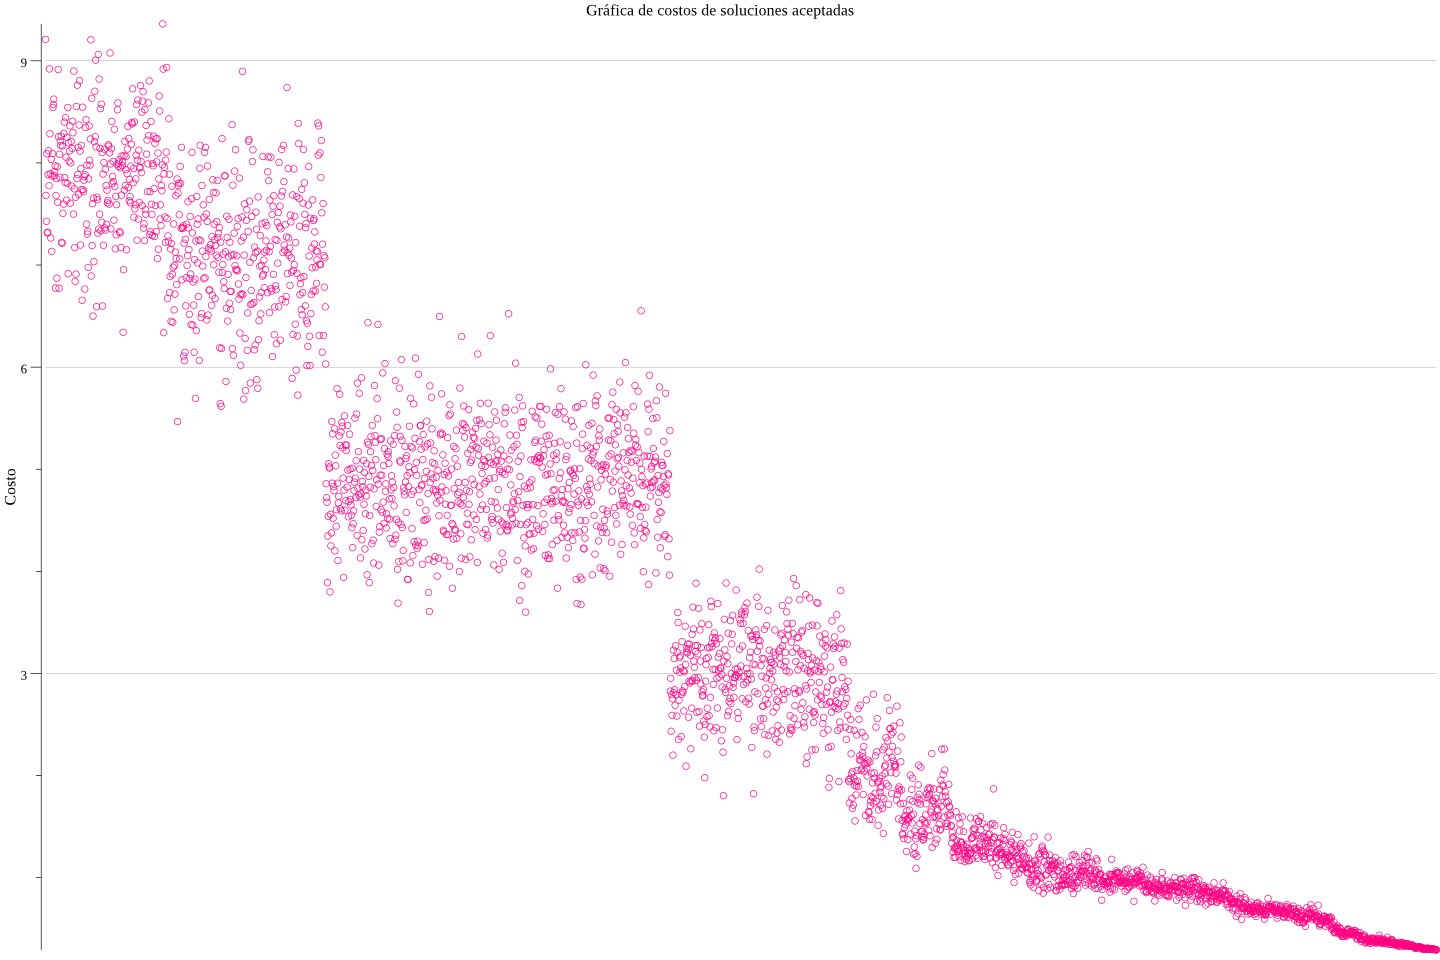
\includegraphics[scale=0.3]{../archivos/graficas/soluciones-aceptadas/costos2.png} \\
\end{center}

El promedio de los costos de las mejores soluciones de todas las semillas fue 0.435944361, lo cuál es una gran mejora del caso anterior. \\

La mejor solución encontrada con Params2 se puede obtener con los parámetros \textsf{archivos/params/2.txt}.

\newpage

\subsubsection*{Params3}

Se obtuvo un $\%$60 de soluciones factibles, poco menos que en el caso anterior. \\

\begin{center}
  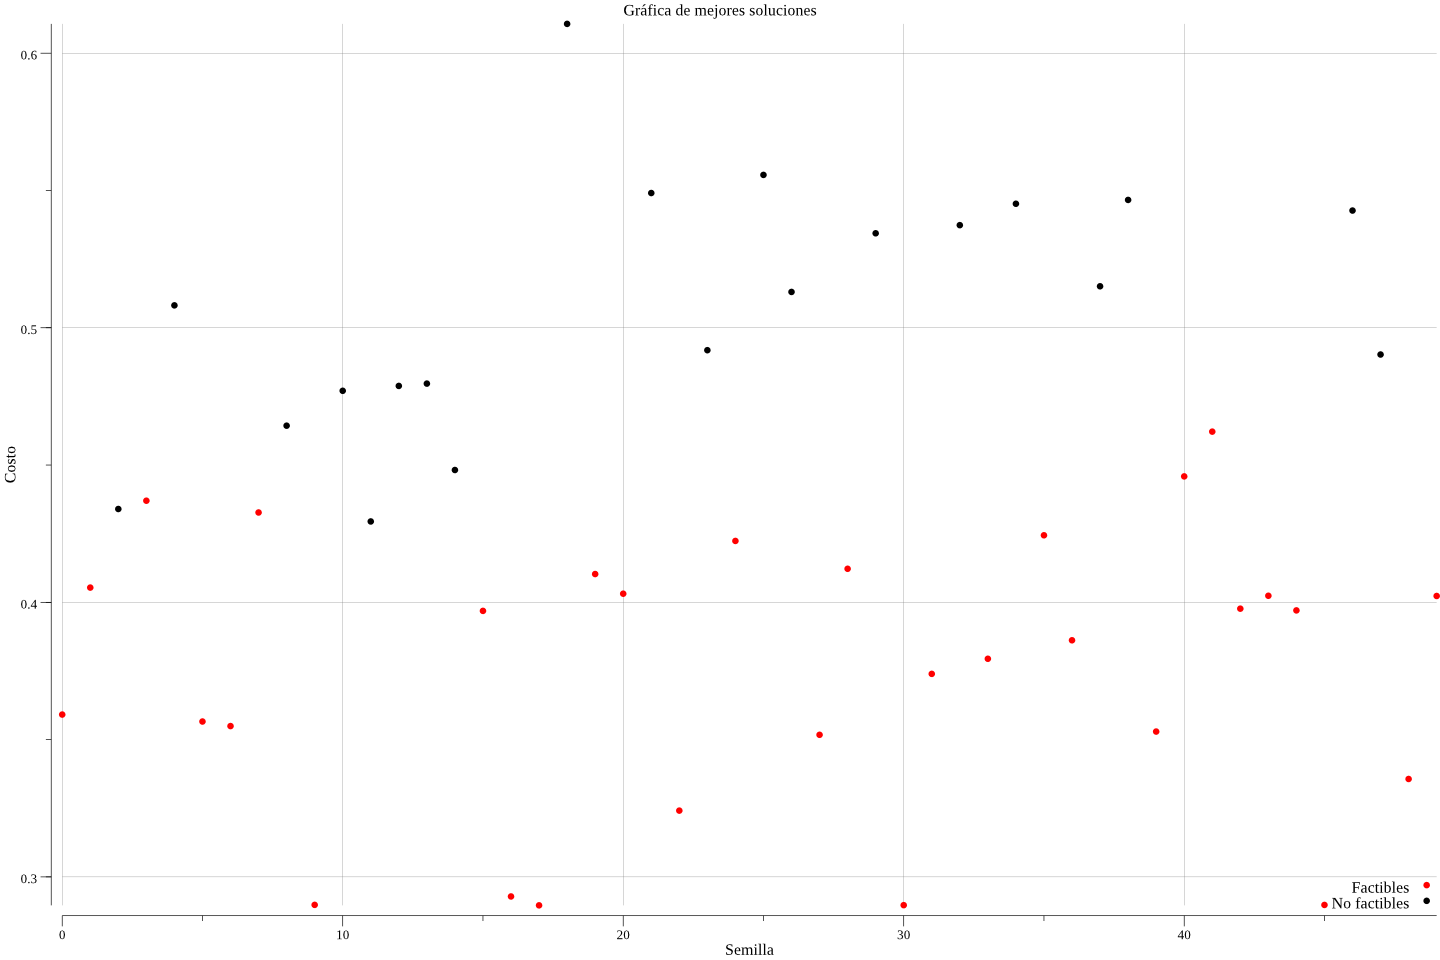
\includegraphics[scale=0.25]{../archivos/graficas/mejores-soluciones/soluciones3.png} \\
\end{center}
  
La mejor solución encontrada tuvo un costo de \textbf{0.289633223}, se obtuvo con la semilla \textbf{17}. Ésta es mejor que la anterior y pareciera ser la óptima, aunque queda la duda. \\

\begin{center}
  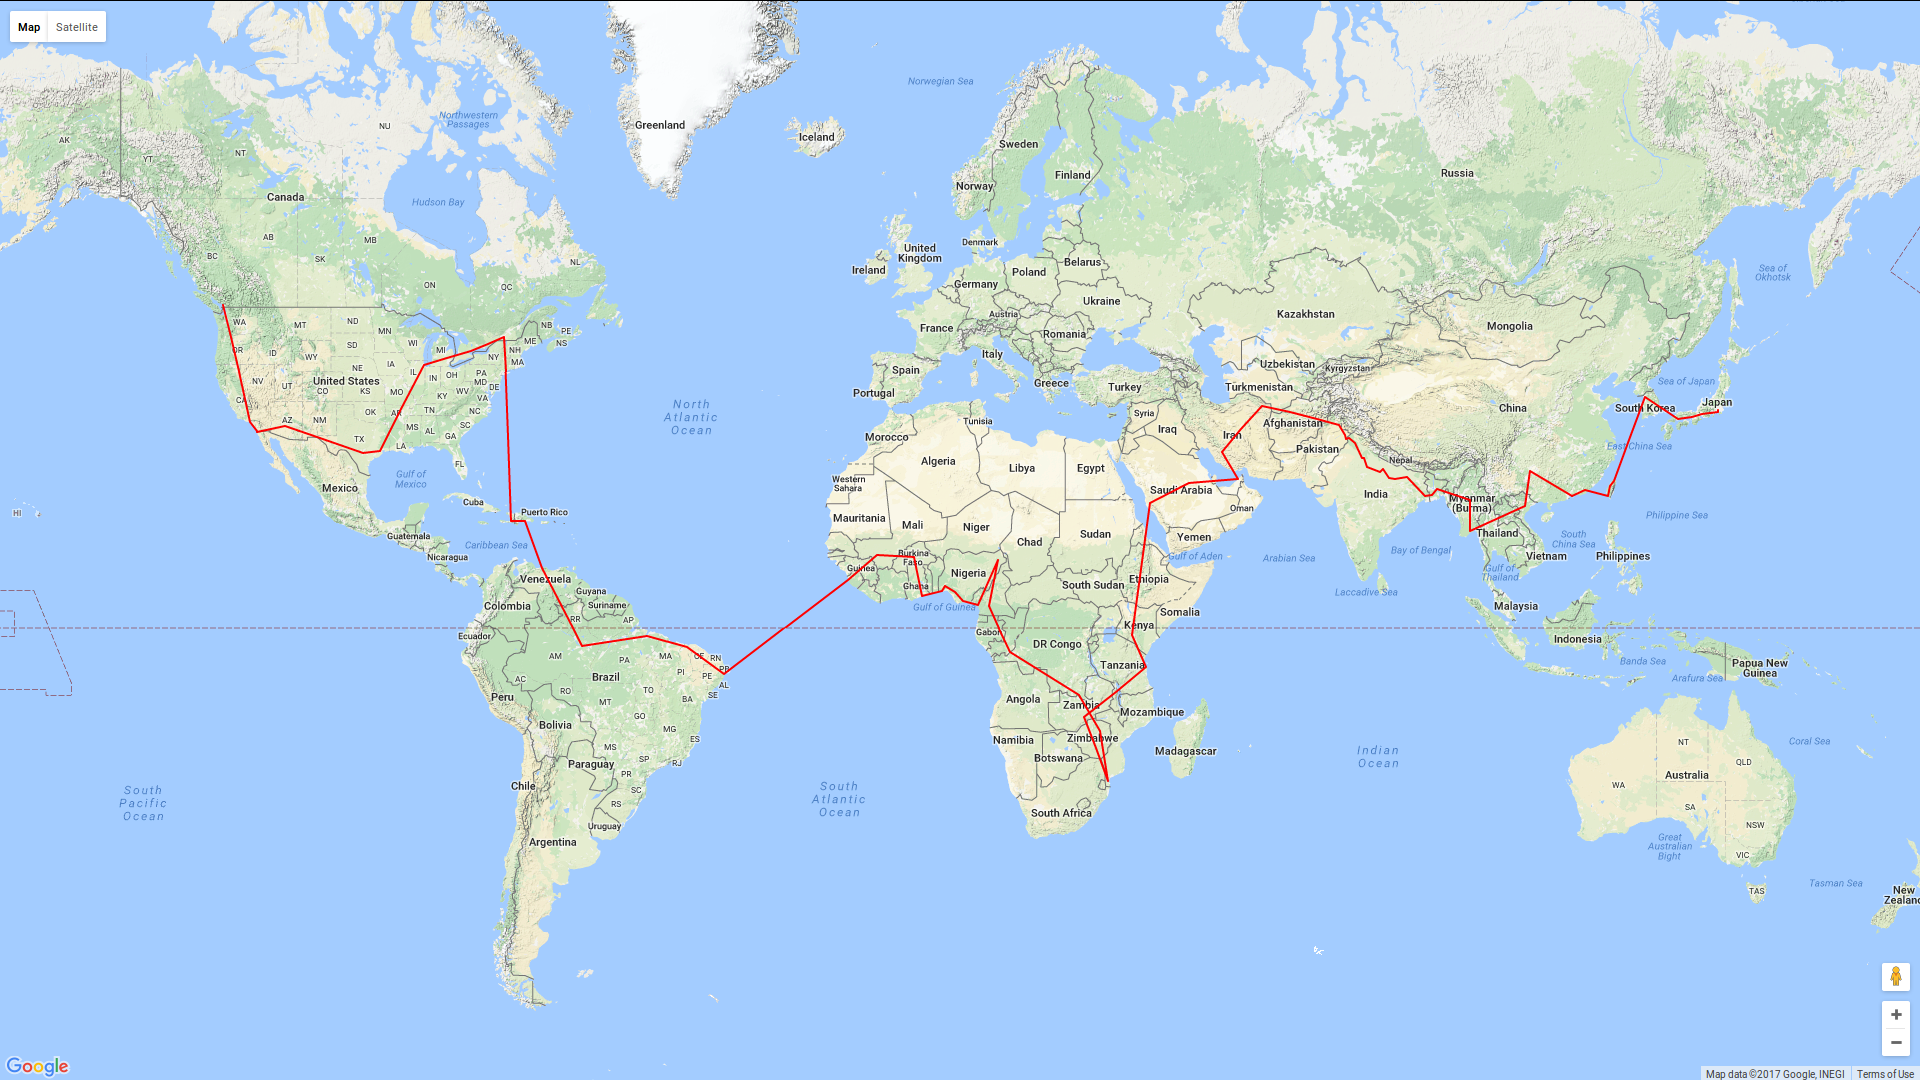
\includegraphics[scale=0.2]{../archivos/mapas/mapa3.png} \\
\end{center}

Gráfica del costo de las soluciones aceptadas de la mejor solución: \\

\begin{center}
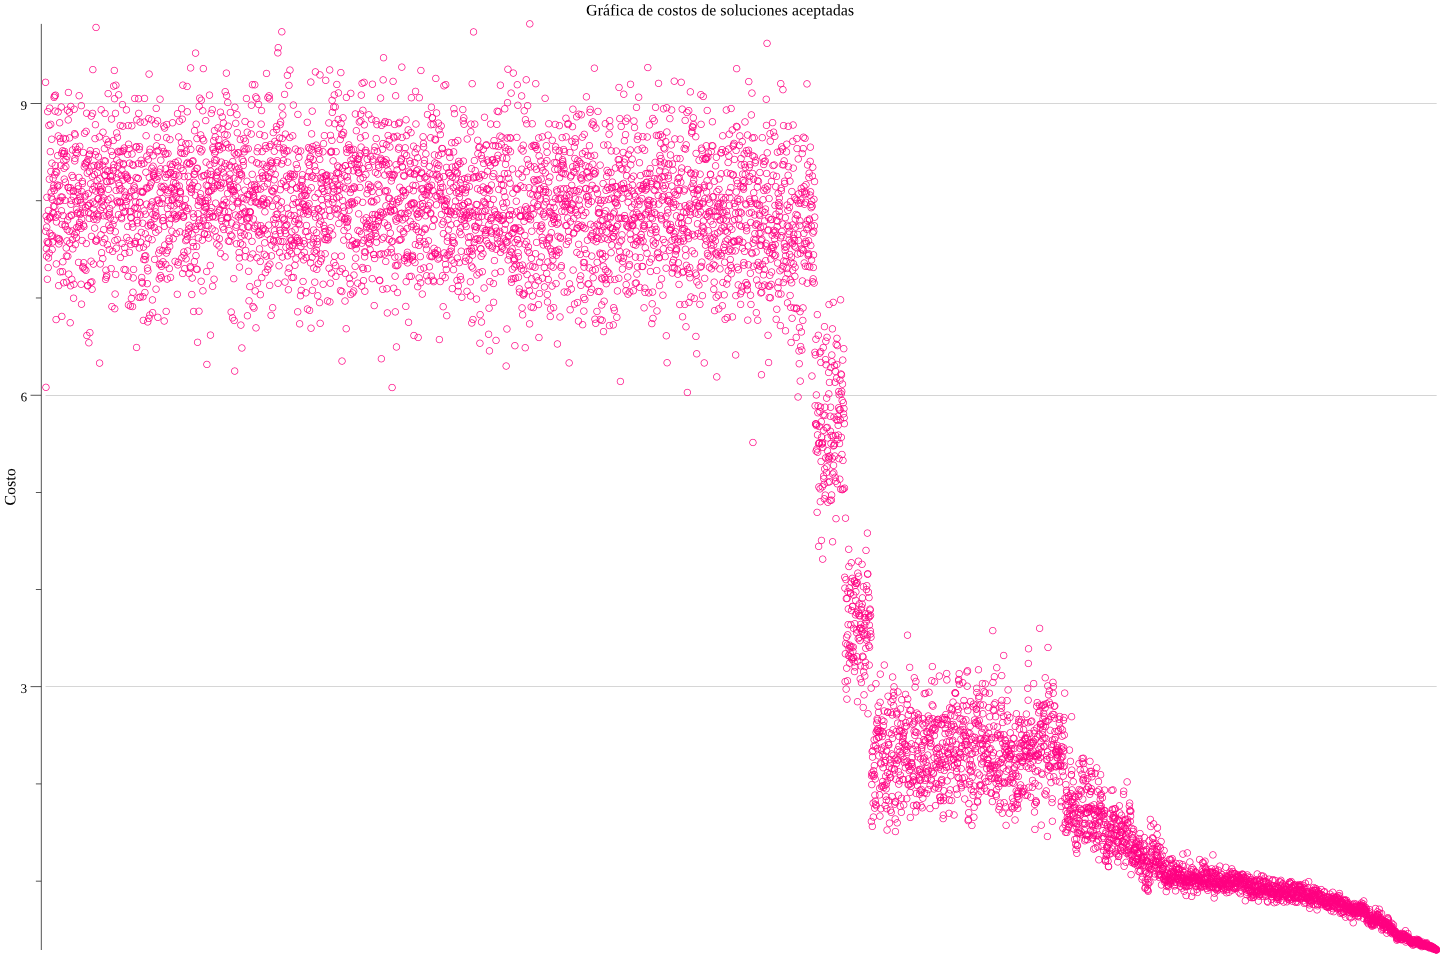
\includegraphics[scale=0.3]{../archivos/graficas/soluciones-aceptadas/costos3.png} \\
\end{center}

El promedio de los costos de las mejores soluciones de todas las semillas fue 0.428595471, muy parecido al caso anterior. \\

La mejor solución encontrada con Params3 se puede obtener con los parámetros \textsf{archivos/params/3.txt}.

\newpage

\subsubsection*{Params4}

Se obtuvo un $\%$76 de soluciones factibles, lo cuál ya es bastante más alto que en los casos anteriores. \\

\begin{center}
  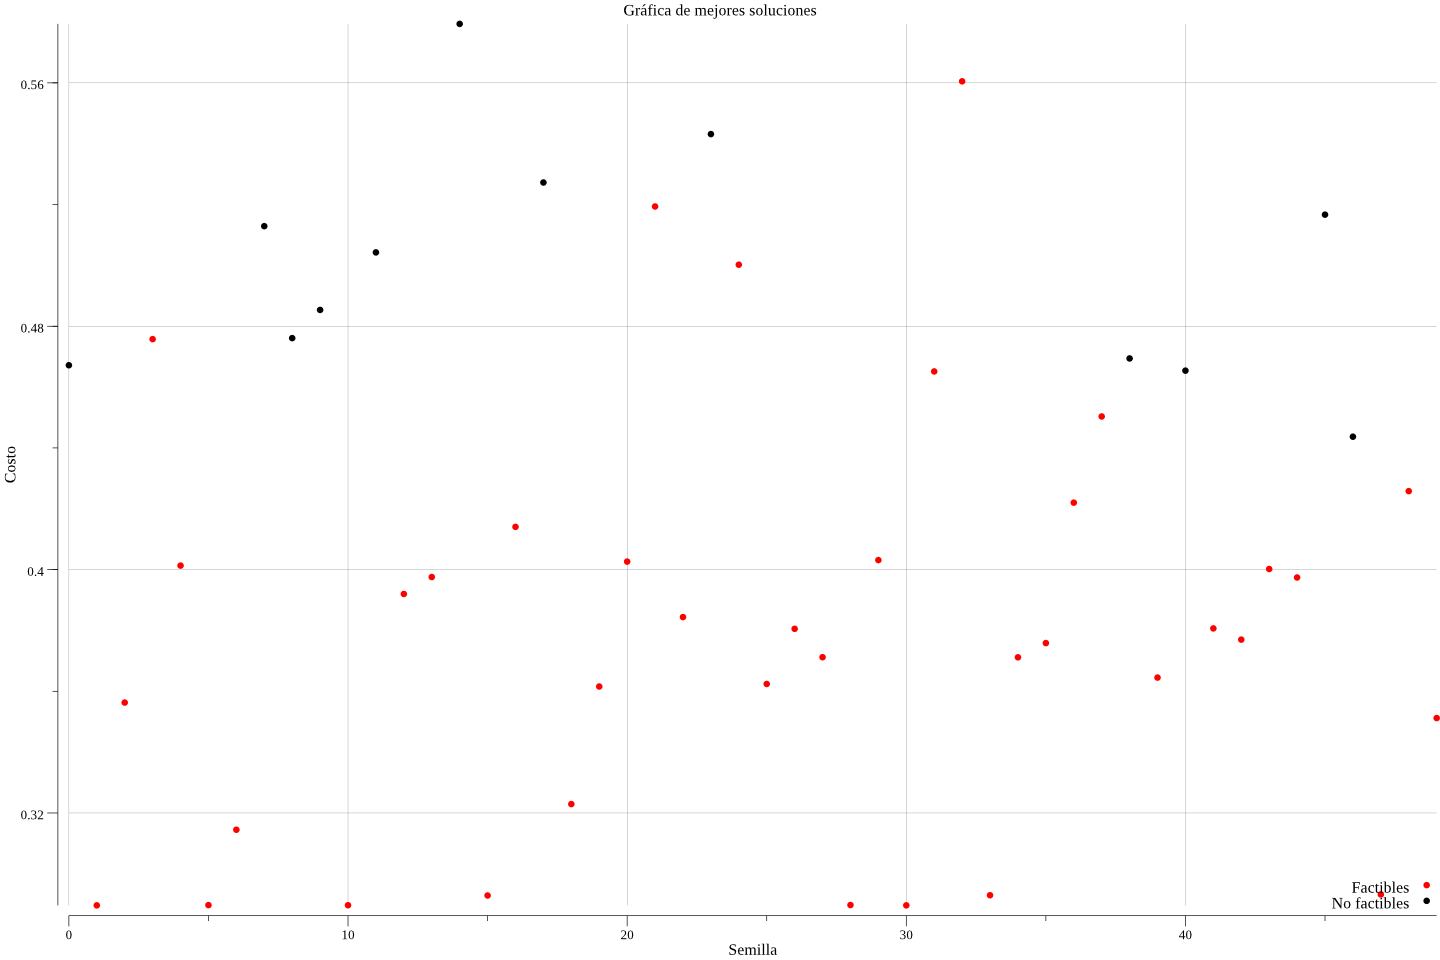
\includegraphics[scale=0.25]{../archivos/graficas/mejores-soluciones/soluciones4.png} \\
\end{center}
  
La mejor solución encontrada tuvo un costo de \textbf{0.289633223}, se obtuvo con la semilla \textbf{1} y la \textbf{30}. Ésta es la misma que en el caso anterior (por ésto se omite el mapa) y la mejor solución obtenida con estos conjuntos de parámetos. \\
Gráfica del costo de las soluciones aceptadas de la mejor solución: \\

\begin{center}
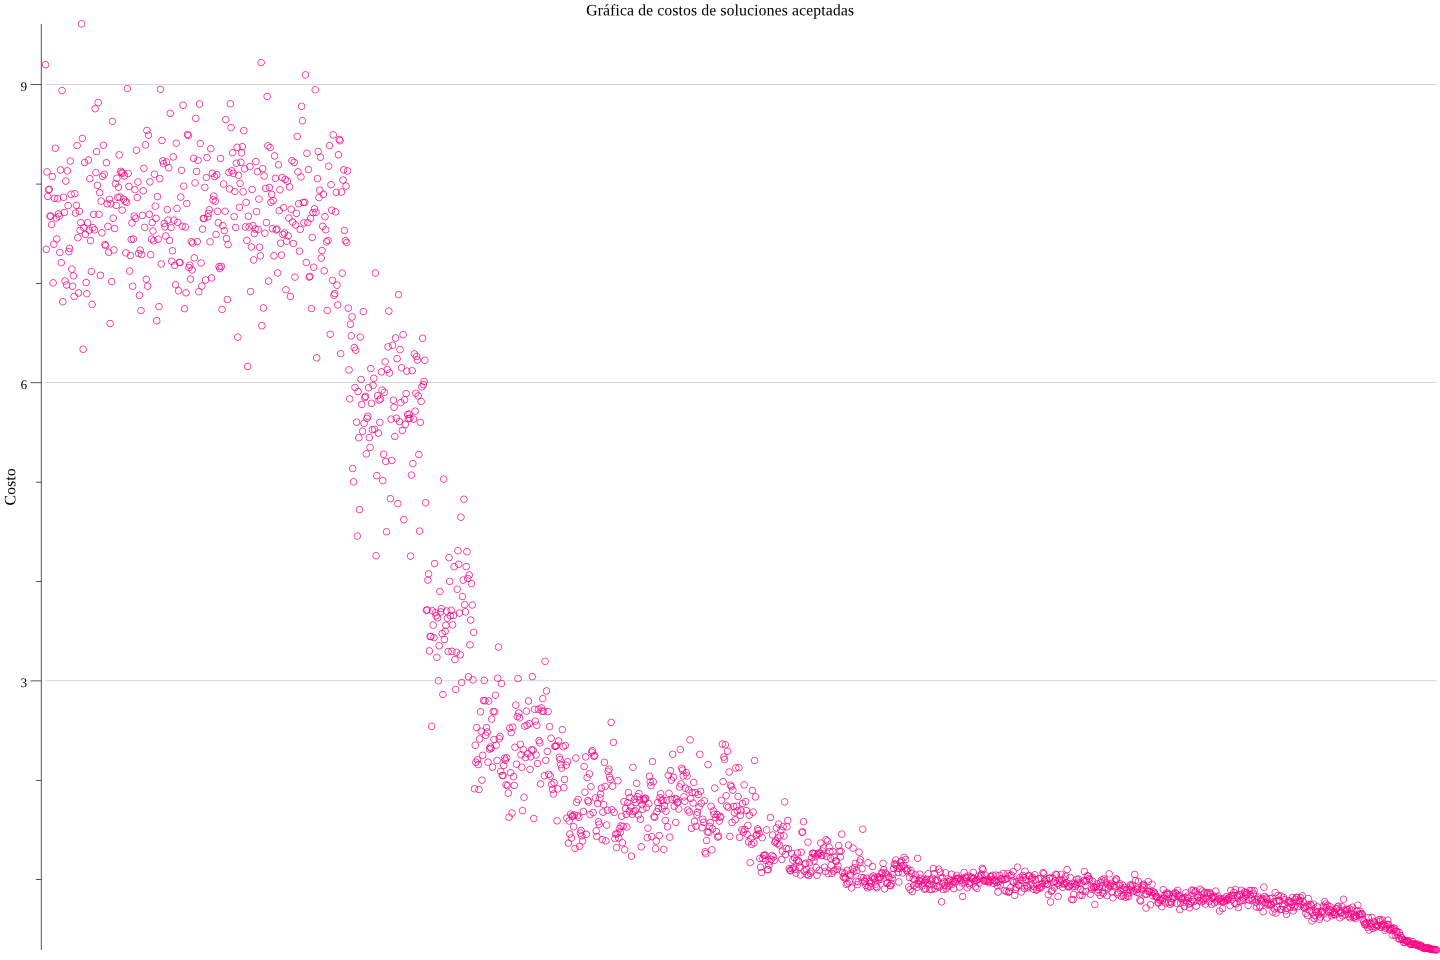
\includegraphics[scale=0.25]{../archivos/graficas/soluciones-aceptadas/costos4.png} \\
\end{center}

El promedio de los costos de las mejores soluciones de todas las semillas fue 0.408394459, lo cuál es una pequeña mejora comparada con los dos casos anteriores. \\

La mejor solución encontrada con Params4 se puede obtener con los parámetros \textsf{archivos/params/4.txt}. \\

Nota: Todas las gráficas se encuentran en \textsf{archivos/graficas} y los mapas en \textsf{archivos/mapas}

\subsection{Conclusiones}

Params1 resultó en soluciones decentes pero lejos de ser las mejores, sin embargo el tiempo de ejecución para cada solución fue bastante menor que con los otros parámetros, ya que las $epsilon$ utilizadas son más grandes en comparación. \\

Con Params2 se pudo obtener una solución muy buena, muy cercana a la óptima y en un número mucho mayor de soluciones factibles, la desventaja es que el programa se tarda más en ejecutarse que con Params1. \\

Params3 y Params4 lograron llegar a una solución que podría ser la óptima, y si no lo es se acerca demasiado. Como es el caso con Params2, la ejecución del programa es bastante más tardada, en especial con Params4, ya que el lote tiene el doble de tamaño que el de los otros casos, sin embargo Params4 logró obtener un porcentaje bastante alto de soluciones factibles. Como podemos ver, mientras perdemos en tiempo ganamos en soluciones, y al contrario. \\

El recocido simulado sirvió muy bien para resolver el problema del agente viajero con el conjunto de ciudades que se nos propuso, el cuál no era muy pequeño pero tampoco muy grande, falta ver que sucede con conjuntos más grandes. \\

La implementación del recocido fue bastante sencilla, sin embargo hay un muchos lugares en los que te puedes perder sin darte cuenta, lo cuál fue mi caso. Go ayudó a que me perdiera en un principio, pero una vez que se le encuentra sentido a este lenguaje, resulta ser una buena herramienta, salvo por algunas cosas subjetivas. \\


\begin{figure}[b]
  
\includegraphics[scale=0.3, right]{../archivos/otros/gopher.png} \\
\end{figure}

\end{document}